\documentclass[10pt,twocolumn,letterpaper]{article}

\usepackage{cvpr}
\usepackage{times}
\usepackage{epsfig}
\usepackage{graphicx}
\usepackage{amsmath}
\usepackage{amssymb}

% Include other packages here, before hyperref.

% If you comment hyperref and then uncomment it, you should delete
% egpaper.aux before re-running latex.  (Or just hit 'q' on the first latex
% run, let it finish, and you should be clear).
\usepackage[breaklinks=true,bookmarks=false]{hyperref}

\cvprfinalcopy % *** Uncomment this line for the final submission

\def\cvprPaperID{****} % *** Enter the CVPR Paper ID here
\def\httilde{\mbox{\tt\raisebox{-.5ex}{\symbol{126}}}}

% Pages are numbered in submission mode, and unnumbered in camera-ready
%\ifcvprfinal\pagestyle{empty}\fi
\setcounter{page}{1}
\begin{document}

%%%%%%%%% TITLE
\title{Automated Attendance System}

\author{Kushal Kumar Jain\\
IIIT - H\\
Gachibowli , Hyderabad\\
{\tt\small kushal.kumar@research.iiit.ac.in}}
% For a paper whose authors are all at the same institution,
% omit the following lines up until the closing ``}''.
% Additional authors and addresses can be added with ``\and'',
% just like the second author.
% To save space, use either the email address or home page, not both


\maketitle
%\thispagestyle{empty}

%%%%%%%%% ABSTRACT
\begin{abstract}
Recording the attendance of a class of more than 50 people at some point in a 90 minutes lecture does not ensure attention of students in the entire lecture. It is almost impossible to ensure someone's attention in the class without monitoring them for the whole duration of the lecture. Hence in this paper I propose a software system which uses a high resolution monitoring camera(s) installed in the lecture hall to identify and track students to record their attendance . The data is easily accessible to the professors and students for future planning and improvement .
\end{abstract}

%%%%%%%%% BODY TEXT
\section{Introduction}


%-------------------------------------------------------------------------
\subsection{The problem}

As attendance is recorded only once when the attendance machines arrive in the class, the class strength rapidly rises and peaks during the time of attendance and falls sharply before and after it. This defeats the purpose of having any attendance at all. The intent behind the minimum attendance policy is to ensure students attention during lectures which the current system is unable to fulfill. Keeping the strength of the class steady at a healthy number is the main problem statement.

\subsection{Current system}

The current system includes many good strategies to improve student attendance in class ~\cite{b1} , like :\begin{enumerate}
\item  Using biometric machines which cannot be easily faked unlike traditional methods under which proxy attendance was a huge issue . \item Linking grades with attendance which automatically transfers the responsibility of high attendance from teachers to students.\end{enumerate}
Although these are good measures but are evidently not enough as very few students remain in the class for the entire duration.\\
In this paper I propose a software system that uses high resolution wide angle camera(s) to identify faces and then track them during the duration of the class, hence calculating the total time the identified object was in the field
of view of the camera ( which is ideally covers the class ) and then rewarding them their attendance.


\section{Literature review}
In my proposed solution we need users to give us their facial data so that they can be recognised and tracked. This data could be used used by Generative One-Shot Face Recognition , or by FaceNet  ~\cite{b2}  ~\cite{b3} . One shot learning based model, requires much less data to be trained as we only get 1-2 photos of the users. We use this as tool that returns us the users name and facial data that we can store and later use to recognize faces. We will also be using Multiple object tracking as a tool that returns all objects identified in the video feed and for how long they were tracked. Here we take an in depth look at both of these tools and the best solution for them that fits our problem statement



%-------------------------------------------------------------------------
\subsection{Object Tracking }

Multiple Object Tracking (MOT) is an important computer vision problem which has gained increasing attention due to
its academic and commercial potential. Although different kinds of approaches have been proposed to tackle this problem, it still
remains challenging due to factors like abrupt appearance changes and severe object occlusions ~\cite{b6}.
\\
For our problem we can use YOLO ~\cite{b4} .It is a novel method to determine bounding boxes as it does not use classifiers, rather uses regression . In this method a single neural network predicts bounding boxes and class probabilities directly from full images in one evaluation. As it is a single network it can be end to end optimized making it extremely fast (45 frames a second). We only need 30 as our standard wide angle video camera would record 30 frames a second.


%-------------------------------------------------------------------------
\subsection{Face Detection}

One-shot face recognition measures the ability to identify persons with only seeing them at one glance, and is a hallmark of human visual intelligence. It is challenging for conventional machine learning approaches to mimic this way, since limited data are hard to effectively represent the data variance. The goal of one-shot face recognition is to learn a large-scale face recognizer, which is capable to fight off the data imbalance challenge. The face recognizer described in the paper ~\cite{b3} by Zhengming Ding, Yandong Guo, Lei Zhang, Yun Fu , is a novel generative adversarial one-shot face recognizer that attempts to synthesize meaningful data for one-shot classes by adapting the data variances from other normal classes.
The other alternative is FaceNet, which provides a unified embedding for face
recognition, verification and clustering tasks. It maps each
face image into a euclidean space such that the distances
in that space correspond to face similarity, i.e. an image ofperson A will be placed closer to all the other images of per-
son A as compared to images of any other person present in
the dataset. The main difference between FaceNet and other
techniques is that it learns the mapping from the images and
creates embeddings rather than using any bottleneck layer
for recognition or verification tasks. 

%-------------------------------------------------------------------------
\section{System Architecture}

Here I describe the main flow of the software system and the functional and non functional requirements that it must fulfill, along with a brief description of its main components.

\begin{figure}
    \centering
    \includegraphics[width=0.8\linewidth]
                   {paper dass.png}
    \caption{UML Class diagram for the system}
    \label{fig:my_label}
\end{figure}
%-------------------------------------------------------------------------
\subsection{Workflow}

\begin{enumerate}
    \item First the Users login using their college IDs and are required to setup their face data using phone camera or webcam.
    \item A logged in user can see his/her enrolled courses and minimum requirement for attendance
    \item When a class begins, the cameras installed in the class start recording and send the video feed to the real time object recognizer module. this module returns all the objects found in the video along with the timestamps of their entry and exit.
    \item this data is sent to the face recognizer module that labels these data and classifies them based on each users face data.
    \item Finally the accumulated attendance is calculated for each object that was recognized as the same person in the video feed.
    \item The total accumulated attendance along with the users ID is sent to the main attendance database after all the edge cases are taken care of manually.The attendance can be given on any scale using any general rule ( for example a score on 1-10 or 1-5 ) that the course instructor may see fit.
    \item Final attendance scores can be viewed by any user at any time for planning purposes.
\end{enumerate}


\begin{figure}
    \centering
    \includegraphics[width=0.8\linewidth]
                   {uml.png}
    \caption{UML use case diagram}
    \label{fig:my_label}
\end{figure}
%-------------------------------------------------------------------------
\subsection{Functional Requirements}
\begin{enumerate}
    \item \textbf {User login :} A safe and secure method to create accounts and authorize logins. College Ids will be used for this purpose as access to college database gives us most of the information we need.
 \item \textbf {Add courses : } Professors can add and delete courses and set the minimum attendance requirement needs along with a scoring system for attendance.
 \item \textbf {Identify objects :} The object identifier module takes the video feed generated by the cameras, as input and gives out a list of all objects detected along with the timestamps.
 \item \textbf {Identify faces :} The face identification module takes the objects recognized by the object recognizer module, as input and gives out the ID of the recognized object and its timestamps as output. 
 \item \textbf{Get Attendance: } The total attendance for each course for a college ID should be easily accessible to the user and this data should be presented to the professor in a manner that promotes improvement in class attendance.
\end{enumerate}
\subsection{Non-Functional Requirements}
\begin{enumerate}
    \item \textbf{Secure Login : } custom passwords or CAS passwords used by the system should be secure and no one other than system administrators or server maintenance personnel should have access to the passwords. 
    \item \textbf{Privacy of face data : } The face data of the users should not be used for malicious purposes , and its privacy should be ensured based on the policy devised by the institute.
    \item \textbf{Privacy of video footages : } Privacy of the video footage must be ensured. These footages should not be used for anything other than recording attendance ( or for purposes agreed upon by the user ).
\end{enumerate}

\subsection{Sequence Diagrams}
sequence diagrams of the following tasks are linked below: 
\begin{enumerate}
    \item Registration and getting attendance data  : Figure \ref{fig:reg}
    \item Calculation of attendance from video feed  : Figure \ref{fig:atten}
\end{enumerate}
\begin{figure}
    \centering
    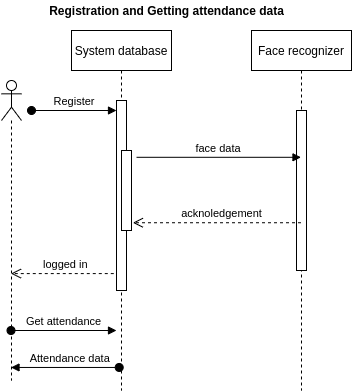
\includegraphics[width=0.8\linewidth]
                   {sequence.png}
    \caption{UML sequence diagram of registration}
    \label{fig:reg}
\end{figure}
\begin{figure}
    \centering
    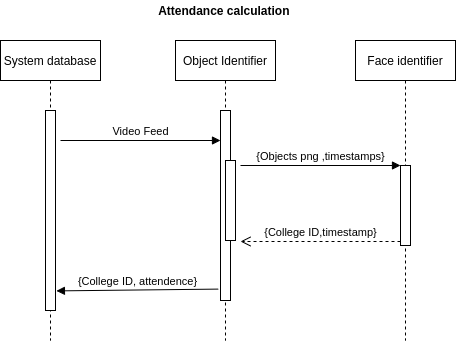
\includegraphics[width=0.8\linewidth]
                   {sequence2.png}
    \caption{UML sequence diagram of calculating attendance from video feed}
    \label{fig:atten}
\end{figure}

\section{Conclusion And Future Work}
In this paper, we successfully proposed a novel software system that uses high resolution camera(s) and face , object identification algorithms to accurately record attendance of students over a 1.5 hour lecture, such that it is almost impossible to not be attend lectures without incurring some penalty. If someone leaves the lecture midway, the timestamps returned by the system for that particular ID, will reflect it in the attendance records. This is not an expensive solution as the only major cost incurred will be that of camera installation, as the rest of the things are managed in software. The accuracy of the solution is as good as the accuracy of face identification module. Hence an accurate face identification module is important. 
For improving this system we can do the following:

\begin{enumerate}
    \item Use more consistent lighting conditions and more data to train our facial recognition module.
    In ideal conditions, facial recognition systems can have near-perfect accuracy. Verification algorithms used to match subjects to clear reference images (like a passport photo or mugshot) can achieve accuracy scores as high as 99.97 on standard assessments ~\cite{b7}
    \item We can have biometric machines as a secondary layer of authentication to further improve the identification process.
    \item We can have pre-defined bounding boxes as the location of tables and chairs can easily be fixed. this reduces our dependence on Object detection algorithms.
    \item we can use cameras near the door to immediately identify and confirm the entry and exits of students more robustly. 
\end{enumerate}




\begin{thebibliography}{00}
\bibitem{b1} "Increase attendance in class" https://www.edsys.in/students-attendance.
\bibitem{b2} Florian Schroff, Dmitry Kalenichenko, James Philbin , "FaceNet: A Unified Embedding for Face Recognition and Clustering", https://arxiv.org/abs/1503.03832
\bibitem{b3}Zhengming Ding, Yandong Guo, Lei Zhang, Yun Fu, ``Generative One-Shot Face Recognition
'' 
\bibitem{b4} Joseph Redmon, Santosh Divvala, Ross Girshick, Ali Farhadi "You Only Look Once: Unified, Real-Time Object Detection"
\bibitem{b5}Nikhil Thakurdesai Nikita Raut, ``Face Recognition using One-shot Learning'' 
\bibitem{b6} Wenhan Luo, Junliang Xing, Anton Milan, Xiaoqin Zhang, Wei Liu, Xiaowei Zhao, Tae-Kyun Kim,
``Multiple Object Tracking: A Literature Review'' 
\bibitem{b7} Comparing rank-1 FNIR at N=1.6M FVRT 2018 mugshot photos for 2020 Yitu-004 algorithm (0.0008) and 2014 NEC-30 algorithm (0.041). Source: Patrick Grother, Mei Ngan, and Kayee Hanaoka, “FRVT Part 2: Identification,” March 27,
\end{thebibliography}

\end{document}
